\documentclass[a4paper,11pt]{article}
\usepackage[margin=1in]{geometry}
\usepackage{tikz}
\usetikzlibrary{positioning, fit, calc}
\usepackage{amsmath}
\usepackage{graphicx}
\graphicspath{{figures/}}

\title{Reliability, Safety and Risk Analysis --- Final Project}
\author{F. Circhetta, P. De Lucia}
\date{\today}

\begin{document}
\maketitle

\begin{abstract}
The aim of this project is to estimate the reliability and availability of a
fairly simple system. Given the complexity involved with Continuous Time
Discrete State Markov Processes - as it is impossible to derive an analytical
solutions when the number of possible states exceeds 4 - time dependent
solutions are obtained through series of indirect Monte Carlo simulations.
\end{abstract}

\section{Introduction}

The system under study is comprised of a 2-out-of-3 system chained in series
with a fourth component. For each of them the failure and repair rates
($\lambda_x$ and $\mu_x$ respectively, $x = A,B,C,D$) are known either by means
of their real value or a specific distribution.

\hspace{2em}

\begin{figure}[ht]
    \centering
    \begin{tikzpicture}[-,auto,node distance=2cm]
        \tikzstyle{point}=[coordinate]
        \tikzstyle{block}=[draw, rectangle, minimum height=2em, minimum width=4em]
        \node[point]  (0)                     {};
        \node[point]  (1) [right of=0]        {};
        \node[block]  (2) [right of=1]        {B};
        \node[block]  (3) [above of=2]        {A};
        \node[block]  (4) [below of=2]        {C};
        \node[point]  (5) [right of=2]        {};
        \node[block]  (6) [right of=5]        {D};
        \node[point]  (7) [right of=6]        {};
        \draw[thick]  (4) -| (1)   (3) -| (1)   (2) -| (1)   (0) -- (1);
        \draw[thick]  (5) |- (2)   (5) |- (3)   (5) |- (4);
        \draw[->,thick] (6) -- (7);
        \draw[->,thick] (5) -- (6);
        \node[draw,circle,thick,dashed,xscale=.5,fit={(2) (3) (4)}] {};
        \node[font=\bfseries,align=center] at (4,-3.2) {2-out-of-3};
    \end{tikzpicture}
    \caption{System under study taken from the project assignment.}
\end{figure}

\section{Assumptions}

\begin{itemize}
    \item System is working at time $t=0$;
    \item No common cause failures;
    \item A component under maintenance is failed;
    \item Every component has its own repair team;
    \item A component, taken individually, can fail even if the system is
    already failed;
    \item Components are continuously monitored and repairs start as soon as the
    component breaks;
    \item The repairs are always successful and bring the component to an ”as
    good as new condition”
\end{itemize}

\section{Algorithm}

\subsection{Input}

Components' transition rates are recorded in a matrix. Then we define the
system's failure logical function (anonymous function of the logical variable
\texttt{state}, which is \texttt{0} if the corresponding component is working or
\texttt{1} if it is failed).

\subsection{Analytical solution (case study 1)}

In order to validate the MC algorithm, the code provides an analytical solution
for reliability and MTTF through the use of the symbolic package.

\hspace{2em}

As for the reliability of the whole system, it is
\begin{align*}
    R^{2oo3}(t) &= R_A R_B R_C + (1-R_A)R_B R_C + R_A(1-R_B)R_C + R_A R_B(1-R_C) \\
    &= e^{-(\lambda_A+\lambda_B)t} +
    e^{-(\lambda_B+\lambda_C)t} +
    e^{-(\lambda_A+\lambda_C)t} -
    2e^{-(\lambda_A+\lambda_B+\lambda_C)t} \\
    R^{sys}(t) &= R^{2oo3}(t) \cdot e^{-\lambda_D t}
\end{align*}

While the equation for the MTTF has been derived as:
\begin{equation}
    MTTF = \int_{0}^{+\infty} t f_T(t) dt = -R(t)t \bigg\rvert_{0}^{+\infty} + \int_{0}^{+\infty} R(t) dt = \int_{0}^{+\infty} R(t)dt
\end{equation}

Once both reliability and MTTF are switched from symbolic to numerical values,
the Monte Carlo simulation can be performed.

\subsection{Reliability and availability}

The simulation relies on the function \texttt{mc\_sim}, which requires as inputs
the components' transition rates matrix, the system's state, the analysis' time
horizon, the number of simulations we want to perform and a logical indicator to
assume (if \texttt{true}) the system definitively failed once it reaches this
state. The function's output will be an array containing: the values on the time
axis, the reliability and its variance, the availability and its variance.

The \texttt{mc\_sim} function performs its computations through the following
operations: in a \texttt{for} cycle iterating a number of times equal to that we
want the simulation to be performed, while the time \texttt{t} is lower than the
mission time, the code will be sampling transition times as
\begin{equation}
    t_2 = t_1 - \frac{\ln(1-R_t)}{\lambda_{state}}
\end{equation}

Where $R_t$ is a random number extracted from a uniform distribution $U(0,1)$,
while $\lambda_{state}$ represents the transition rate of the system out from
its current configuration and has been computed as the sum of all of the
components' transition rates.

\hspace{2em}

Now the affected component has to be found. To do so, given that the transition
occurs at the sampled time \texttt{t}, the transition probabilities for each
component will be
\begin{equation}
    p_k = \frac{\lambda^k_{tr}}{\lambda_{state}}, k = 1, 2, \ldots, \#components
\end{equation}

These probabilities will then be compared with a random number (again extracted
from a uniform distribution $U(0,1)$) to determine which component will be
subject to transition. Once the affected component is found its state has to be
switched and will simply have to be switched to the opposite state since the
components in the given system can only be in one state at the time and, when
repair is a possibility, each of them is continuously monitored and repaired
right after failure by a dedicated maintenance team.

\hspace{2em}

The code then checks if the components' transition has led to system failure
otherwise if the system previously was in a failed state. If the system has
failed a lower time boundary is set at the first instant greater or equal to the
transition time and thereon the system failure counters are increased, and so
the simulation may start over again. If, on the other hand, maintenance is a
possibility, the code will set an upper boundary for the down-time and account
for the instantaneous unavailability through the use of counters. Reliability
and availability (and their variance) can be calculated as the complementary
functions of unreliability and unavailability, which have been found by applying
the Monte Carlo integration method.

\subsection{Average availability}

The average availability is computed as the integral mean of the instantaneous
availability over the mission time span

\begin{equation}
    q_{T_p} = \frac{1}{T_p} \int_0^{T_p}q(t)dt
\end{equation}

\subsection{MTTF}

We move to computing the MTTF through a Monte Carlo simulation. This calculation
will be performed by a function similar to the previous employed for the
reliability, but it will simply account for failure times in an array when the
simulation results in a failed state. The MTTF is then computed following the
Monte Carlo integration method together with its variance

\begin{equation}
    MTTF = \int_0^{+\infty}tf_T(t)dt
\end{equation}

To finish off, the code performs a last Monte Carlo simulation computing trials
for the MTTF to provide information on the validity of the results obtained
through validation at 1, 2 and 3-$\sigma$ level of confidence.

\subsection{Uncertainty on parameters}

The last point we'll focus on is the Monte Carlo simulation of reliability and
availability with a Bayesian approach when the real value of some parameters is
unknown. In this case, we know the parameters are distributed according to a
lognormal distribution. First of all, we'll need to move from logarithmic mean
and variance to exact ones. To do so, given logarithmic mean values ($m_i$) and
coefficient of variation ($cv$), we will perform the following calculations:

\begin{equation}
    var_i = {\left(cv \cdot m_i \right)}^2 ,
    \mu_i = \ln \left(\frac{m_i^2}{\sqrt{var_i\cdot m_i^2}}\right),
    \sigma_i = \sqrt{\ln\left(\frac{var_i}{(m_i^2+1)}\right)}
\end{equation}

These calculations give the correct parameters to employ in the log-normal
random sampling of the two failure rates in the external loop, where they are
iteratively substituted in the components' characteristics matrix to be employed
by the Monte Carlo simulation function previously described to compute the
reliabilities and availabilities together with their variances, in accordance
with the following procedure:

\begin{equation}
    R(t) = P(T>t) = \int_0^{+\infty} P(T>t|\lambda)p''(\lambda|E)d\lambda = \int_0^{+\infty} R(T|\lambda)p''(\lambda|E)d\lambda
\end{equation}

Where $p''$ is the posterior distribution of the failure rate given the event
$E$, which, while unknown, allows us to consider $\lambda$ distributed as a
lognormal.

\section{Results}

\subsection{Case study 1: no repair}

In the case of no available maintenance the system will most likely be failed at
mission time ($\sim21$ days), with a value within the 95\% confidence interval
[$0.032342$; $0.034618$], since the single components present MTTFs of 200, 250,
333 and 1000 hours, respectively, giving an overall MTTF of system in the 95\%
confidence interval [$181.50h$; $183.25h$].

\begin{figure}[ht]
    \centering
    \begin{minipage}{.5\textwidth}
        \centering
        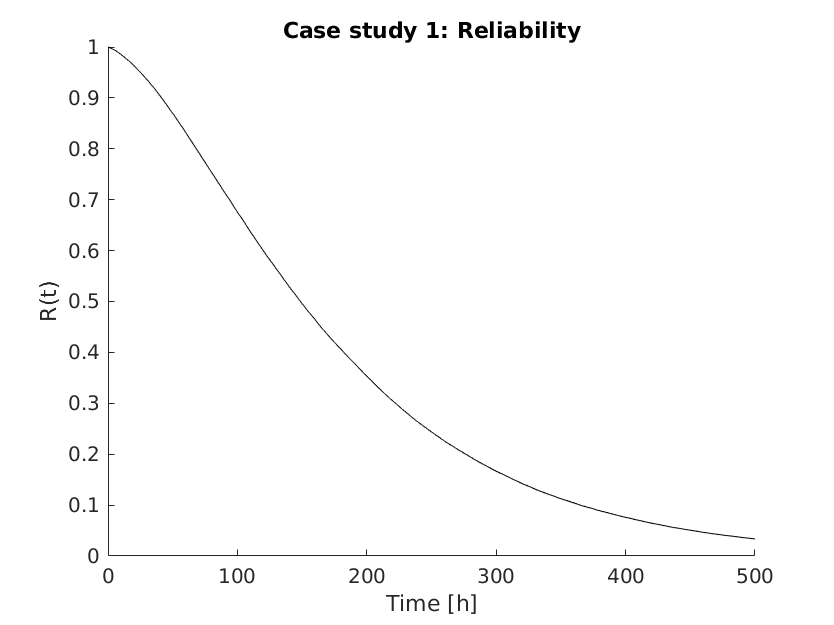
\includegraphics[width=1\linewidth]{Rel1.png}
        \caption{Time dependent reliability $R(t)$}
    \end{minipage}%
    \begin{minipage}{.5\textwidth}
        \centering
        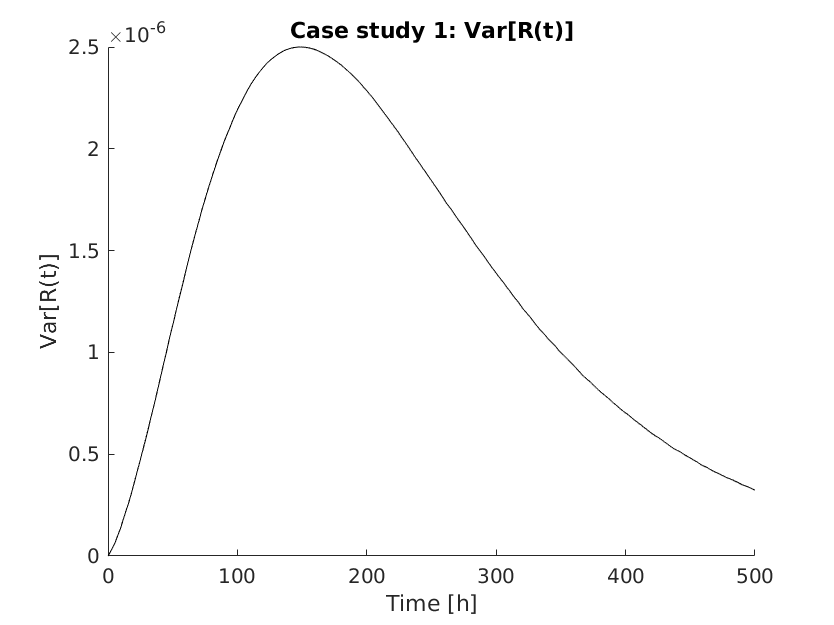
\includegraphics[width=1\linewidth]{Rel1_var.png}
        \caption{Time dependent $R(t)$ variance}
    \end{minipage}
\end{figure}

For the first point of the project, we were able to validate the MTTF and
reliability values over multiple trials given the analytical solution, the
obtained results are satisfactory.

\begin{figure}[h!]
    \centering
    \begin{minipage}{.5\textwidth}
        \centering
        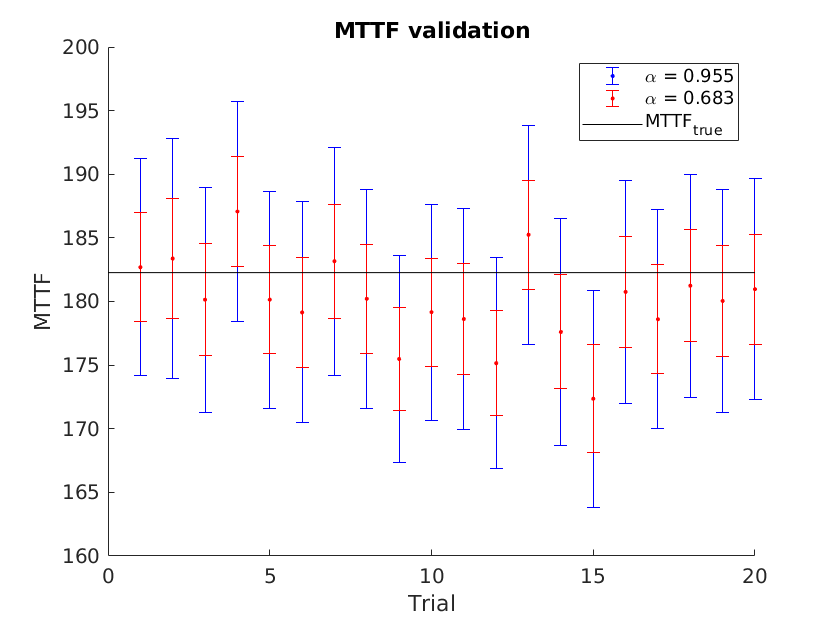
\includegraphics[width=1\linewidth]{MTTF_val.png}
        \caption{$MTTF$ validation}
    \end{minipage}%
    \begin{minipage}{.5\textwidth}
        \centering
        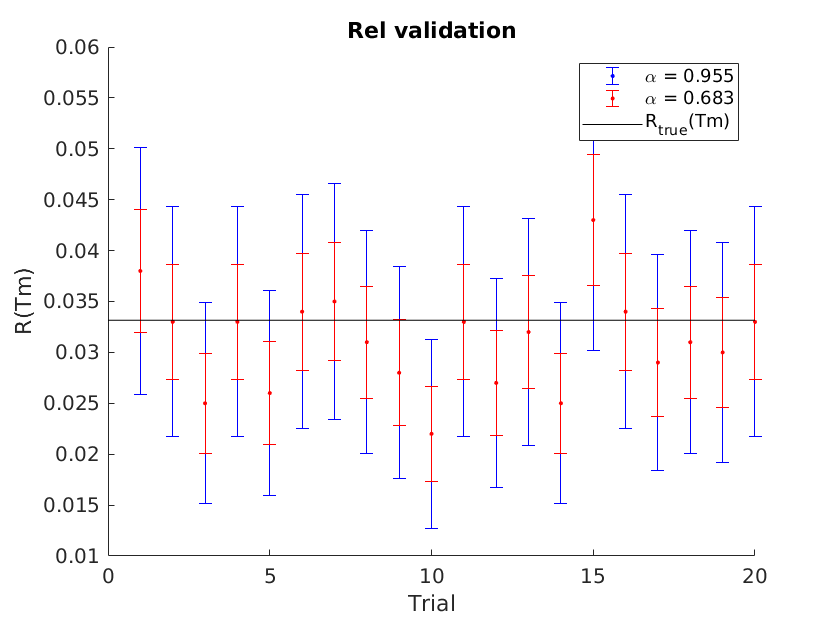
\includegraphics[width=1\linewidth]{Rel_val.png}
        \caption{$R(500h)$ validation}
    \end{minipage}
\end{figure}

\subsection{Case study 2: repairs allowed}

Introducing the possibility of maintenance, the reliability curve of the system
will be decreasing more slowly, and with a value within the 95\% confidence
interval: [0.39168; 0.39787]. What actually is more relevant in this analysis is
the trend shown by the availability, which, after a brief transition period,
reaches an equilibrium around a stationary value. The mean availability in the
mission time, in the 95\% confidence interval, will be [0.99151; 0.99152],
giving a mean downtime of $\sim$4.23 h. In this case the MTTF lies in the 95\%
confidence interval [$532.42h$; $539.14h$].

\begin{figure}[ht]
    \centering
    \begin{minipage}{.5\textwidth}
        \centering
        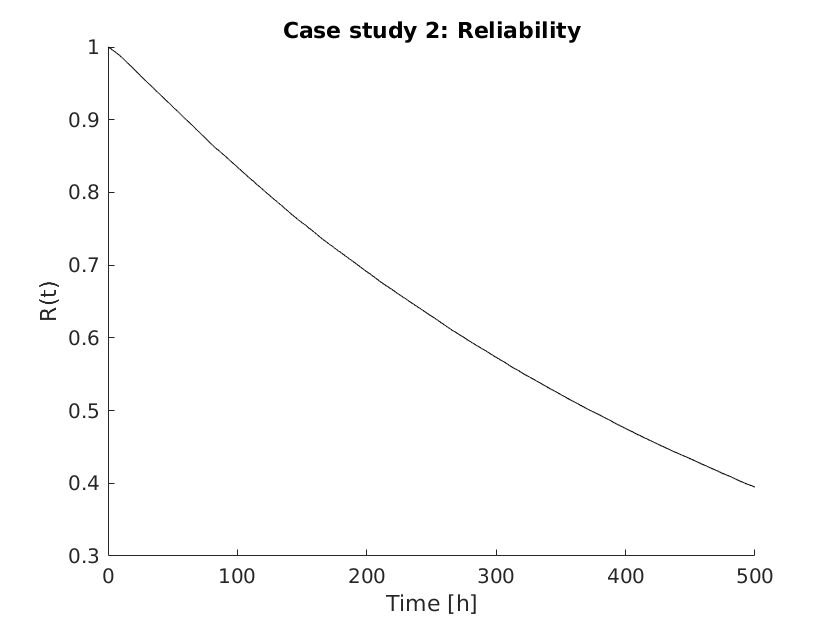
\includegraphics[width=1\linewidth]{Rel2.png}
        \caption{Time dependent reliability $R(t)$}
    \end{minipage}%
    \begin{minipage}{.5\textwidth}
        \centering
        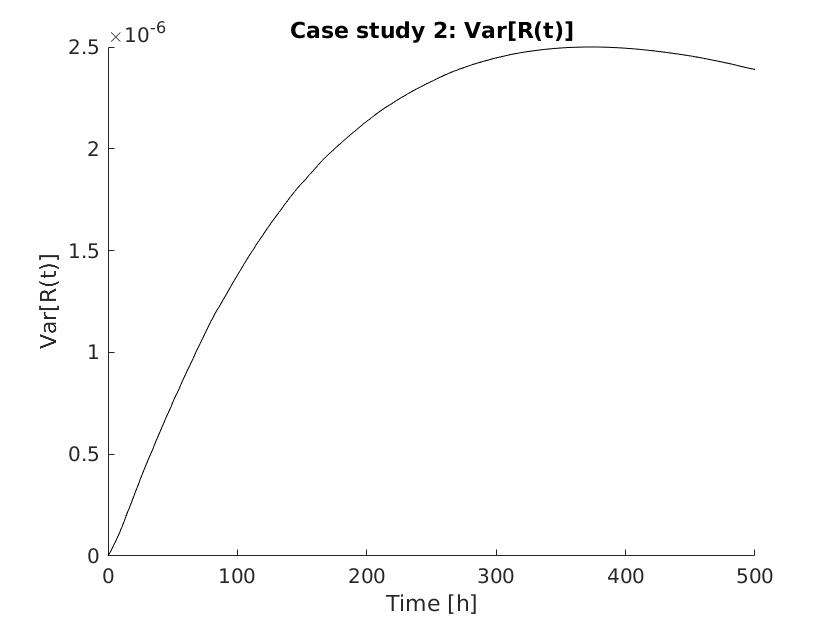
\includegraphics[width=1\linewidth]{Rel2_var.png}
        \caption{Time dependent $R(t)$ variance}
    \end{minipage}
\end{figure}

\begin{figure}[ht]
    \centering
    \begin{minipage}{.5\textwidth}
        \centering
        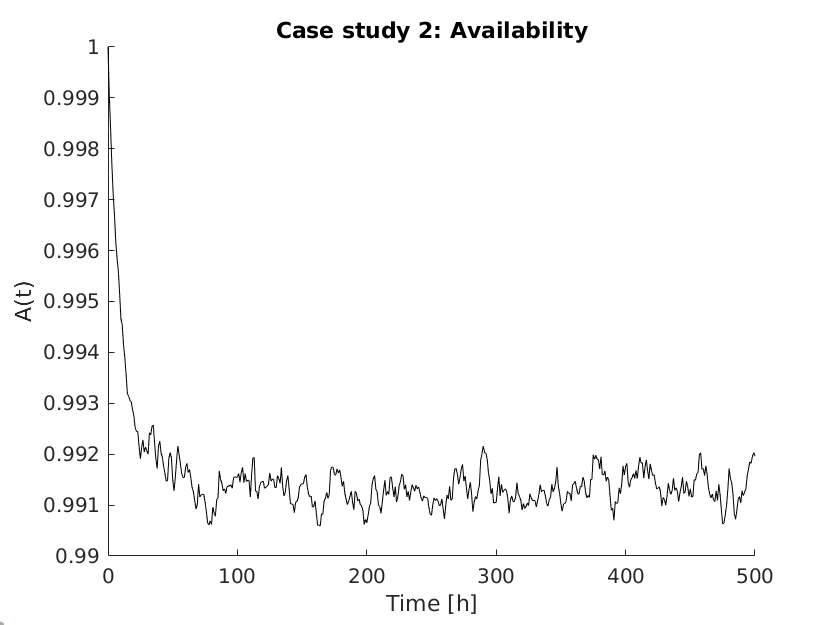
\includegraphics[width=1\linewidth]{Avail2.png}
        \caption{Time dependent availability $A(t)$}
    \end{minipage}%
    \begin{minipage}{.5\textwidth}
        \centering
        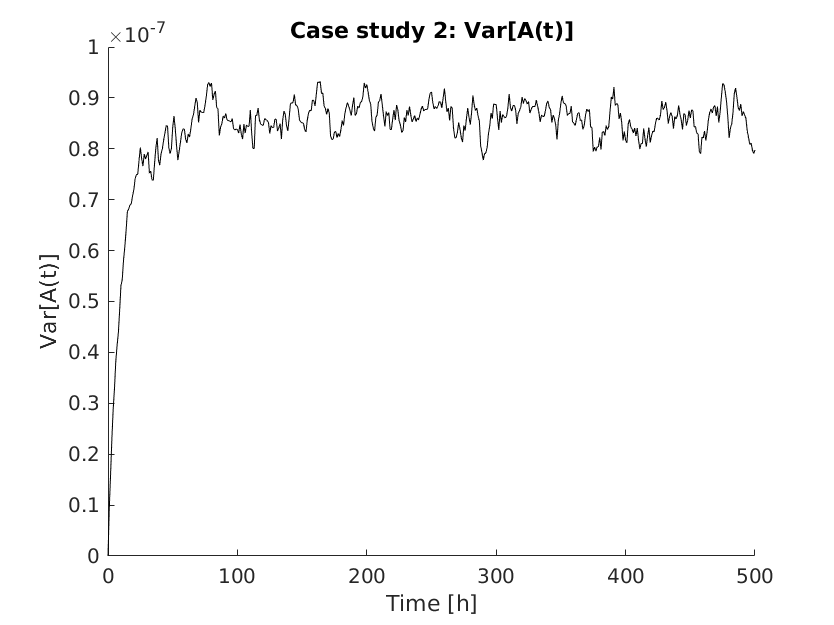
\includegraphics[width=1\linewidth]{Avail2_var.png}
        \caption{Time dependent $A(t)$ variance}
    \end{minipage}
\end{figure}

\subsection{Case study 3: Bayesian framework}

As for point three of the project, the mean values assigned to the two failure
rates were the same as the real ones for the previous analysis, so we didn't
expect much change amongst the results. The Bayesian framework provides us with
an analytic value for reliability and availability, even though the parameters
presented are uncertain; this wouldn't have been the case if we were to employ
the frequentist framework.

\begin{figure}[ht]
    \centering
    \begin{minipage}{.5\textwidth}
        \centering
        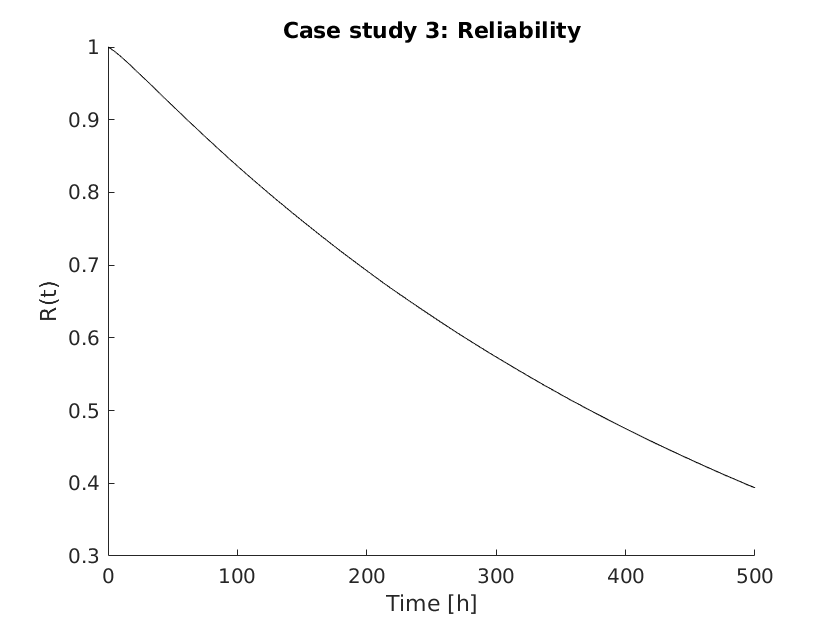
\includegraphics[width=1\linewidth]{Rel3.png}
        \caption{Time dependent reliability $R(t)$}
    \end{minipage}%
    \begin{minipage}{.5\textwidth}
        \centering
        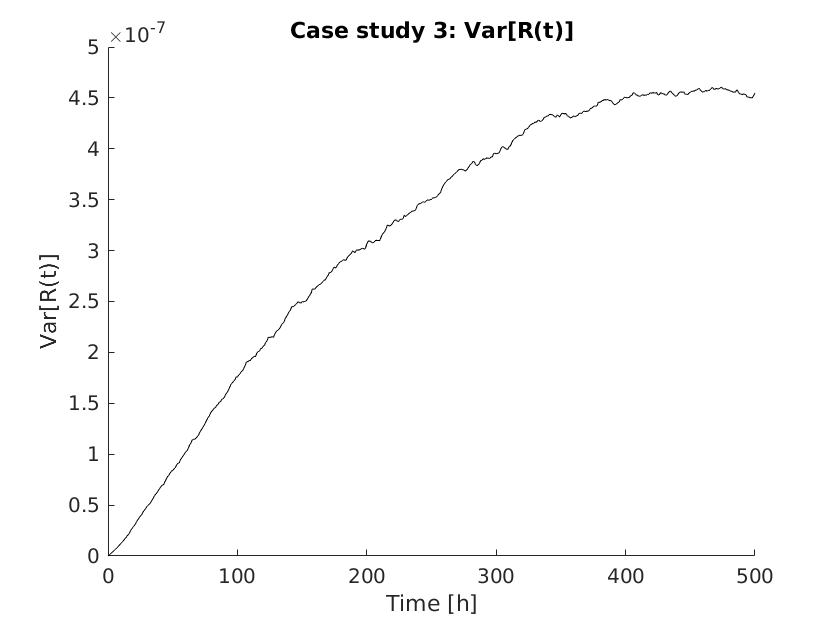
\includegraphics[width=1\linewidth]{Rel3_var.png}
        \caption{Time dependent $R(t)$ variance}
    \end{minipage}
\end{figure}

\begin{figure}[ht]
    \centering
    \begin{minipage}{.5\textwidth}
        \centering
        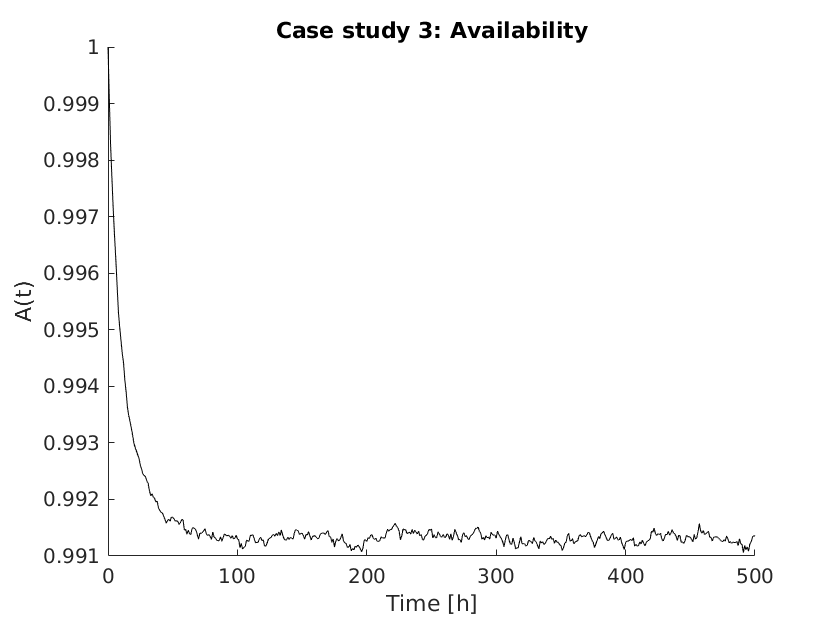
\includegraphics[width=1\linewidth]{Avail3.png}
        \caption{Time dependent availability $A(t)$}
    \end{minipage}%
    \begin{minipage}{.5\textwidth}
        \centering
        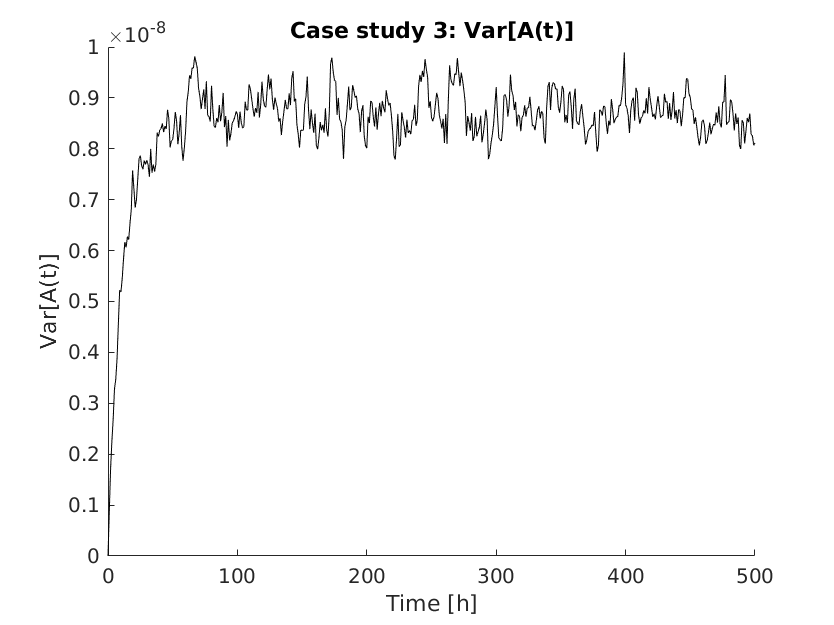
\includegraphics[width=1\linewidth]{Avail3_var.png}
        \caption{Time dependent $A(t)$ variance}
    \end{minipage}
\end{figure}

\end{document}
